\chapter{Descripci\'on de las configuraciones radiol\'ogicas en simulaciones Monte Carlo}

El presente capítulo se trata sobre una breve introducción a códigos de simulación Monte
Carlo dedicados al transporte de radiación. Se presentan las características genéricos de
los códigos PENELOPE y FLUKA. La exposición se enfoca en la posibilidad de realizar
aplicaciones en radiodiagnóstico.

\section{Introducción y par\'ametros en la simulación del transporte de radiaci\'on}

Como se mencionó en las secciones precedentes, los métodos Monte Carlo son una forma genérica para denominar procedimiento matemáticos cuya característica común es el uso de números generados aleatoriamente y distribuciones de probabilidad. En la actualidad el método Monte Carlo es ampliamente aceptado y cada vez mas extendido, como una herramienta para realizar investigación científica, específicamente para modelar el transporte de radiación en medios materiales.

En muchos casos de interés en el campo de rediodiagnóstico, como una situación particular del transporte de radiación, el método Monte Carlo es el más apropiado, ya que no se dispone de métodos alternativos de carácter experimental, anlítico y/o instrumental.

\section{Setups virtuales}

El método Monte Carlo puede resultar fácilmente aplicable a sistemas con geometrías complejas y diferentes medios materiales. De hecho, éste método permite simular el paso de la radiación a través de la materia tomando en cuenta todos los procesos físicos relevantes y todos los tipos de radiación involucrados, como tipo de partículas (electrones, positrones, fotones, neutrones, iones pesados y partículas como muones, kaones, etc) que pueden ser simulados hasta que se detengan.

En términos genéricos, el armado de la configuración de irradiación requiere de definir la fuente de radiación (en propiedades físicas y geométricas), la muestra que es irradiada (en geometría y propiedades físicas), los sistemas de etección, con las propiedades definidas por el usuario, así como determinar cuáles son los procesos, y bajo qué critarios, se consideran en la simulación.

A modo de fijar ideas, se presenta el diseño del set up de uuna situación típica en radiodiagnóstico, como es la simulación de un tubo de rayos X:

\begin{quote}
La geometría que debe simularse para el proceso de producción de rayos X se corresponde con el dispositivo típico de un tubo de rayos X. En primer lugar, se define la fuente de electrones mediante ( por ejemplo mediante fuentes puntuales ubicadas a lo largo de una longitud de 2 mm). Los electrones viajan en l’inea recta hacia el ánodo de material (por ejemplo, tungsteno con espesor de 0.5 mm y ángulo de inclinación de unos 10 - 15 grados). Cuando los electrones ingresan en el material blanco el programa simula la trayectoria de los electrones hasta que éstos finalmente llegan al “reposo” o a una situación terminal. Durante los procesos de interacción se considera la producción de rayos X característicos y Bremsstrahlung. Los fotones que emergen del blanco atraviesan la envoltura de vidrio pirex de 0.5 mm de espesor, y finalmente el filtro adicional de aluminio de 1 mm de espesor. 
\end{quote}

El espectro calculado representa el número de fotones por intervalo de energía en función de la energía. Los resultados pueden ser obtenidos con los códigos PENELOPE o FLUKA, entre otros.

\section{Ejemplos de c\'odigos de simulaci\'on Monte Carlo para transporte de radiaci\'on}

Existen disponibles varios códigos de simulación dedicados a modelar el transporte de radiación. Algunos de los códigos más utilizados en aplicaciones de física médica son MCNP, EGS4, GEANT4, PENELOPEy FLUKA.

En general, los código de simulación Monte Carlo construyen un modelo estocástico en base a funciones de densidad de probabilidad modelando secuencialmente eventos individuales de una variable aleatoria. Es decir, teóricamente se siguen todos los eventos o interacciones que sufre cada partícula desde su origen hasta que alcanza una condición terminal (absorción, escape, energía de corte, etc). 

Para cualquier evento, los códigos de simulación generan un número aleatorio fundamentándose en las funciones de densidad de probabilidad, que definen el tipo de interacción y otros parámetros. Posteriormente, se calcula el valor esperado de todos los eventos simulados.

Para realizar una simulación, debe crearse un archivo de entrada, típicamente denominado “input”. Este archivo contiene de manera estructurada información sobre el problema en aspectos tales como la geometría del problema, materiales utilizados, secciones eficaces a utilizar, la localización y características de la fuente y los tipos de resultados que se desea obtener de la simulación.

\subsection{El c\'odigo PENELOPE v. 2008}

El código PENELOPE refiere a PENetration and Energy LOss of Positrons and Electrons (luego se incorporaron fotones).

Algunas de las principales caracteríaticas son:

\begin{itemize}
 \item Cascadas acopladas de tipo “fotón-electrón”.
 \item Transporte de fotones por medio de simulación detallada, que refiere a computar evento por evento.
 \item Transporte de electrones/positrones por medio de simulación mixta, i.e. en combinación entre simulación detallada y técnicas denominadas “simulación condensada”, que consisten básicamente de implementar criterios para acumular una serie de eventos en único evento equivalente -estadísticamente-. Para ello, se cuenta con formalismos teóricos denominados multiple scattering theory.
 \item El rango de energía disponible en PENELOPE es 50 eV a 1 GeV.
 \item Las partículas secundarias que se generan son simuladas en orden cronológico.
\end{itemize}

Existen, cuatro estructuras o bloques principales:

\begin{itemize}
 \item {\bf Input:} Se requiere de un archivo de inicialización para ingresar los datos de entrada.
 \item {\bf Modelado de eventos de colisión:} Simulación de interacciones.
 \item {\bf Algoritmos internos de cómputo:} Rutinas numéricas asociadas al proceso de cómputo.
 \item {\bf Modelo de tracking:} Transporte de la radiación.
\end{itemize}

Al iniciar la simulación, PENELOPE lee el archivo de input, realiza la simulación y, como resultado, crea archivos nuevos de salida denominados “outputs”, que incluyen los resultados generados, estimaciones para los errores producidos y algunas tablas que resumen el proceso de simulación.

La figura \ref{figPENELOPE} muestra esquemáticamente el diagrama de flujos del código PENELOPE.

\begin{figure}
 \centering
 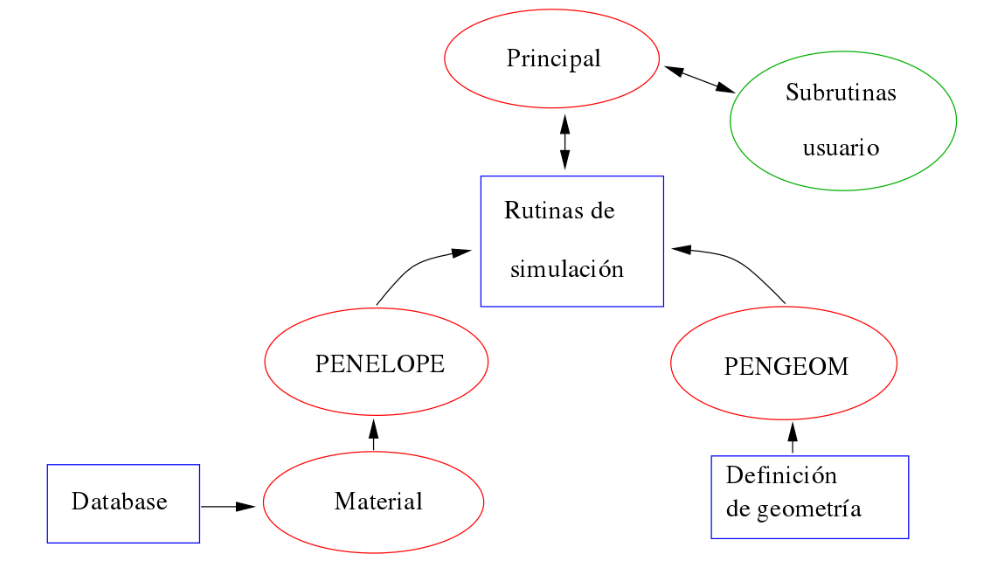
\includegraphics[width = .75\textwidth]{figures/cap7/penelope.png}
 \caption{Diagrama esquemático de la estructura de PENELOPE.}
 \label{figPENELOPE}
\end{figure}

La base de datos de PENELOPE cuenta con 279 materiales, entre elementos puros y
compuestos.

\subsection{El c\'odigo FLUKA v. 2011}

El proyecto FLUKA pertence al CERN, y es desarrollado para propósitos de física de partículas de alta energía, alcanzando valores de hasta varias decenas de TeV, o incluso mayores con linking a nuevas librerías restringidas.

En términos generales, FLUKA is un paquete integral de simulación de física de partículas. Cuenta con varios campos de aplicación que incluyen, entre otros, física teórica y experimental de alta energía, ingeniería, diseño de infraestructuras y protecciones (shielding), diseño de telescopios y detectores, estudios de rayos cósmicos, dosimetría, física médica y radiobiología.

En cuanto a su capacidad, brevemente FLUKA puede simular con gran precisión todos los procesos de interacción y propagación de más de sesenta tipos de partículas, entre ellas fotones y electrones, neutrinos, muones de varias cantidades de energía, hadrones, así como de sus correspondientes antipartículas.

La figura \ref{figFLUKA} muestra esquemáticamente el contenido central del paquete FLUKA.

\begin{figure}
 \centering
 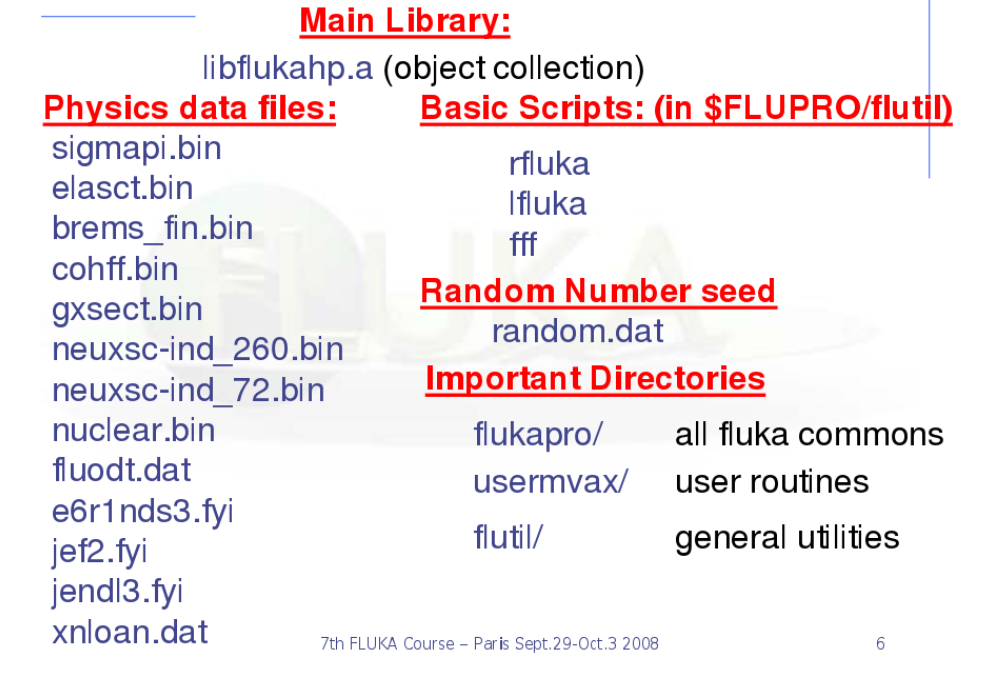
\includegraphics[width = .75\textwidth]{figures/cap7/fluka.png}
 \caption{Contenido básico de FLUKA.}
 \label{figFLUKA}
\end{figure}

